\section{Runtime complexity on large scale reconstructions}
In practice, Coordinate Descent gets used together with heuristics, which improve its runtime complexity. Pinning down the average runtime of Coordinate Descent is difficult, because we need an estimate of how well the heuristics work on average. For our algorithm, the runtime mainly depends on the number of non-zero starlet components $S$ and how many iterations Coordinate Descent needs to converge. How many non-zero starlets, or how many iterations Coordinate Descent needs on average are hard questions and cannot be answered in this project.

Instead, this work focuses on a minimum runtime estimate of Coordinate Descent on MeerKAT observations. We compare the runtime complexity with WSCLEAN and analyse what speed up an idealized version of Coordinate Descent can provide. Sadly, the speed up of an idealized Coordinate Descent is negligible. The Major Cycle architecture leads to a lower runtime complexity in the context of MeerKAT reconstructions.


\subsection{Runtime complexity of an idealized Coordinate Descent}
The runtime complexity of Coordinate Descent depends largely on the number of Visibilities $M$ and the number of non-zero starlets $S$. The number and location of the $S$ non-zero starlets are generally not known. However, we created a heuristic which finds likely non-zero starlet components. In a realistic setting, the heuristic will have found more than $S$ likely non-zero starlets. For the idealized version of Coordinate Descent, we assume an oracle performance heuristic: It finds the location and number of the $S$ non-zero starlet components in constant time ($O(1)$). Coordinate Descent therefore has to find the value of $S$  components. In total, the idealized Coordinate Descent algorithm has four operations: creating J starlet levels with the non-uniform FFT, creating the columns of $F^{-1}$, calculating the minima for each single component, and calculating the starlet layers:

\begin{alignat*}{1}
J \text{non-uniform FFTs for the starlet regularization} &: J*(M + 2N*ld(2N))\\
\text{creating} \:S\: \text{columns of}\: F^{-1} &: S*7M\\
\text{locating} \:S\: \text{minima of} \:S\: \text{parabolas} &: S*4M\\
\text{calculating} \:J\: \text{Starlet layers} &: J * 2M
\end{alignat*}

We assume we have enough memory to cache the columns of $F^{-1}$ and only need to calculate them once. Coordinate Descent arrives at the correct result in $I_{CD}$ iterations. Therefore we arrive at the runtime complexity of \eqref{results:cd:omega}.

\begin{equation}\label{results:cd:omega}
\begin{aligned}
	CD(I_{CD}, M, S, J) = &I_{CD} * [S * 4M + J * 2M]\\
		&+  S*7M\\
		&+ J*(M + 2N*ld(2N))
\end{aligned}
\end{equation}

Note that the runtime of Coordinate Descent is independent of the number of pixels. The only image related parameter in \eqref{results:cd:omega} is $J$, the number of starlet layers. The largest starlet layer represents the largest possible structure in the image, which is given by the instrument and the image resolution (pixels per arc-second). The runtime only depends indirectly on the image resolution, not the total number of pixels.

Also note the term iterating over the $S$ non-zero starlets, $ I_{CD} * [S * 4M +\ldots]$. As it turns out, this is the Achilles heel of the algorithm. MeerKAT observations contain a very large amount of Visibilities $M$.

\subsection{Runtime complexity of WSCLEAN}
We look at WSCLEAN reconstructions which use the non-uniform FFT with $w$-stacking. The runtime of a single Major cycle depends on the non-uniform FFT with $w$-stacking and the number of CLEAN deconvolutions. $N$ denotes the number of pixels.

\begin{alignat*}{1}
	\text{non-uniform FFT} &: M + 2N*ld(2N)\\
	\text{non-uniform FFT with} \:w\text{-stacking} &:M + W*(2N*ld(2N) + 2N) + N*ld(N)\\
	I_{WSCLEAN}\: \text{deconvolutions} &: I_{WSCLEAN}*2N
\end{alignat*}

The overall complexity shown in \eqref{results:clean:o} can also be split into two parts. In each Major Cycle, the forward and backwards non-uniform FFTs gets calculated, and CLEAN deconvolves the image for a certain number of iterations.

\begin{equation}\label{results:clean:o}
\begin{aligned}
 WSCLEAN(I_{Major}, I_{CLEAN}, M, N,  W) =\: &I_{Major} * 2 * [M + W*(2N*ld(2N) + 2N) + N log N]\\
	&+ I_{Major} * [I_{CLEAN}*2N]
\end{aligned}
\end{equation}

Notice that the number of CLEAN deconvolutions $I_{CLEAN}$ depends on the image content, similar the number of non-zero starlets $S$ for Coordinate Descent. Here however, it multiplies with the number of pixels $N$ instead of the number of Visibilities $M$. In a sense, the major cycle tries to reduce the runtime complexity of handling the image content by calculating the non-uniform FFT. If the difference is large enough $N \ll M$, then the Major Cycle will end up with a smaller overall runtime.


\subsection{Comparison on a MeerKAT reconstruction problem}
Our real-world MeerKAT observation has been calibrated and averaged in frequency and time, to reduce storage space. The resulting dataset contains 540 channels with 4 million Visibilities each. The uncalibrated dataset contains 8 times more Visibilities. First we estimate the runtime complexity on the calibrated and averaged dataset. The size of the uncalibrated data becomes relevant for the second estimate, where we compare WSCLEAN and Coordinate Descent in the self-calibration setting.

For our first estimate, we same values needed for the WSCLEAN reconstruction in image \ref{scale:wsclean}:
\begin{itemize}
	\item Visibilities: $M=2.19e^9$
	\item $w$-stacks: $W = 128$
	\item Pixels: $N = 8192^2$
	\item Maximum number of CLEAN iterations: $I_{CLEAN} = 35'000$
\end{itemize}

For the runtime estimate of WSCLEAN, we assume it requires $I_{Major}=10$ Major Cycles to converge. CLEAN reconstructions tend to use around five Major Cycles. Compressed sensing reconstructions, which use the Major Cycle framework, tend to use around 10 cycles. It puts our WCLEAN runtime estimate in the area of current compressed sensing reconstructions, and is a very favourable assumption for Coordinate Descent.

The idealized Coordinate Descent algorithm has three parameters left: Number of starlet levels $J$, number of non-zero starlets $S$, and number of iterations to converge $I_{CD}$. We under-estimate and set $J=5$, assuming the largest structure in the image is no more than 160 pixels in size. With these assumptions, we plug in the values into the equations \eqref{results:cd:omega} and \eqref{results:clean:o}, and compare the runtime for different values of $S$ and $I_{CD}$ in table \ref{scale}

\begin{table}[h!]
	\begin{center}
		\begin{tabular}{l|c|c|c|c} % <-- Alignments: 1st column left, 2nd middle and 3rd right, with vertical lines in between
			 & $I_{CD} = 1$ & $I_{CD} = 5$ &  $I_{CD} = 10$ &  $I_{CD} = 15$\\
			\hline
			$S=1000$ & 2.34 & 0.96 & 0.55 & 0.38 \\
			$S=2000$ & 1.17 & 0.48 & 0.27 & 0.19\\
			$S=3000$ & 0.78 & 0.32 & 0.18 & 0.13\\
			$S=4000$ & 0.59 & 0.24 & 0.14 & 0.1\\
		\end{tabular}
		\caption{Relative speed-up of an idealized Coordinate Descent compared to CLEAN.}
		\label{scale:cd:table}
	\end{center}
\end{table}

To put the numbers into perspective, Coordinate Descent used about 2000 non-zero starlets to reconstruct the image \ref{results:mixed:cd}. Since the reconstruction does not contain all point sources, the true number of $S$ is likely to be higher than 2000 on a simulated dataset with simple, Gaussian extended emissions. A MeerKAT reconstruction can contain more complex emissions. Image \ref{scale:wsclean} shows the WSCLEAN reconstruction of the current observation. We see a large number of small, point-like objects and several complex extended emissions. We need at least 2000 non zero starlet components to represent the MeerKAT image. In the best case scenario, when the ideal Coordinate Descent converges within one iteration, we have a 17\% runtime improvement over CLEAN. Keep in mind that we have over-estimated the runtime of CLEAN.

\begin{figure}[h]
	\centering
	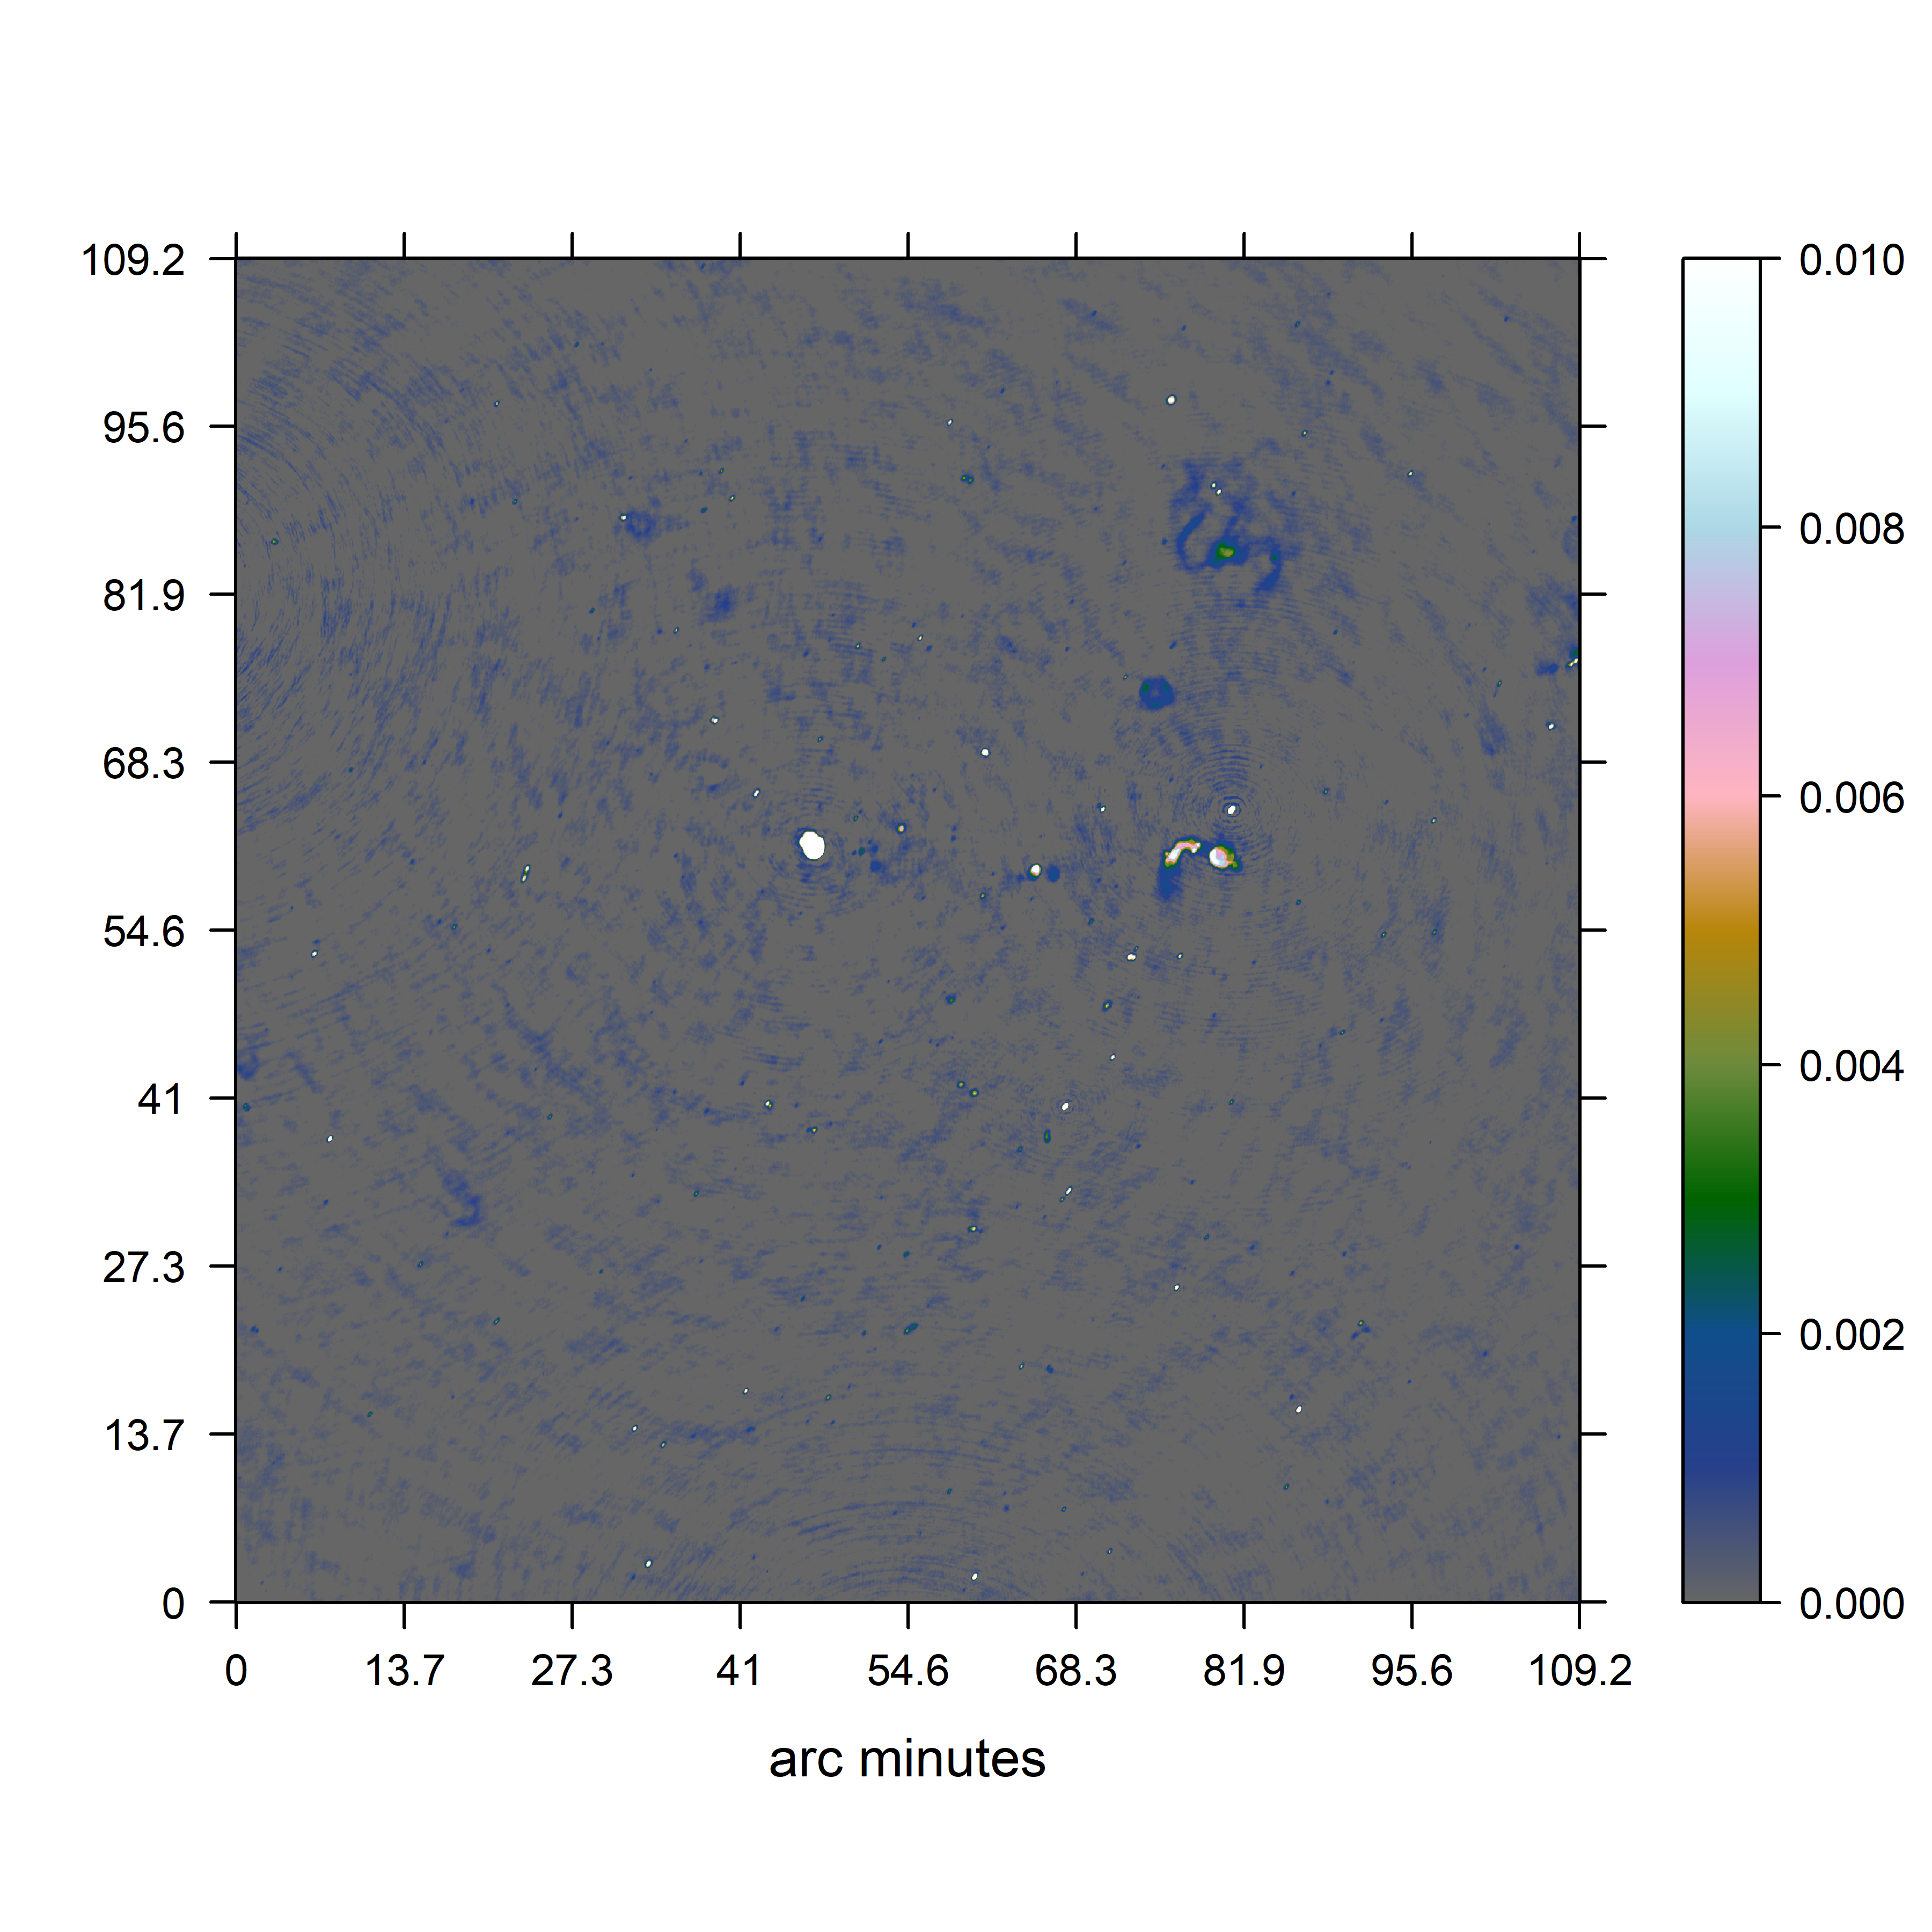
\includegraphics[width=0.6\linewidth]{./chapters/21.scalability/meerkat.png}
	\caption{WSCLEAN Reconstruction of the MeerKAT observation.}
	\label{scale:wsclean}
\end{figure}

So far, we have excluded the memory requirement of Coordinate Descent from our analysis. A short glance at the numbers reveals it is impractically large. A single column of $F^{-1}$ has $M$ entries, effectively multiplying the number of Visibilities with each column we need to cache. With 2000 starlets, we may not need 2000 columns. Several starlets may be at the same pixel location, but at different scales. In this estimate, we used $J=5$ levels. In the best case, we need just 400 pixels to arrive at 2000 starlets. Still, this results to 12 terabytes of memory minimum just for the columns alone, when we use 128bit accuracy for complex valued Visibilities. 

There is one last question, for which Coordinate Descent could be useful: Since the runtime complexity \eqref{results:cd:omega} scales independently of the image size $N$, maybe it offers a speed up if we want to reconstruct very large images. Let us scale up the image by a factor of 16, to $N=32768^2$ and compare the speed up to WSCLEAN in table \ref{res:cd:large:table}. 

\begin{table}[h!]
	\begin{center}
		\begin{tabular}{l|c|c|c|c} % <-- Alignments: 1st column left, 2nd middle and 3rd right, with vertical lines in between
			& $I_{CD} = 1$ & $I_{CD} = 5$ &  $I_{CD} = 10$ &  $I_{CD} = 15$\\
			\hline
			$S=1000$ & 37.91 & 15.56 & 8.96 & 6.29 \\
			$S=2000$ & 19.1 & 7.81 & 4.49 & 3.15  \\
			$S=3000$ & 12.76 & 5.21 & 3 & 2.1  \\
			$S=4000$ & 9.58 & 3.91 & 2.25 & 1.58 \\
			\hline
			$S=10000$ & 3.84 & 1.57 & 0.9 & 0.63  \\
			$S=15000$ & 2.56 & 1.04 & 0.6 & 0.42\\
			$S=20000$ & 1.92 & 0.78 & 0.45 & 0.32 \\
		\end{tabular}
		\caption{Relative speed-up of Coordinate Descent compared to CLEAN with an image size of $N=32000^2$. }
		\label{res:cd:large:table}
	\end{center}
\end{table}

Note that the speed up is roughly linear to the pixels per Visibility ratio. We increased the pixels by a factor of 16, and table \ref{res:cd:large:table} is approximately the result of 16 multiplied by table \ref{scale:cd:table}. The Coordinate Descent approach sees considerable speed up, if it converges within one iteration. But it falls off quickly as soon as it needs several iterations to converge. Any realistic Coordinate Descent algorithm cannot move far away from the minimum estimate of the ideal before it gets more expensive than our WSCLEAN estimate. However, there is another point to consider: An image of this size will have a high resolution coupled with a wide field of view. In this scenario, we would likely want to improve the image with self-calibration. At this point, we need the uncalibrated, raw Visibilities for imaging, which increases $M$ again by a factor of 8. By including self-calibration, any speed up of table \ref{scale:cd:table} gets approximately divided by 8. Again, Coordinate Descent is again only competitive if it needs just 1 iteration to converge.  

The issue with Coordinate Descent's runtime complexity lies in the term $I_{CD} * [S * 4M +\ldots]$ of \eqref{results:cd:omega}, which scales with the "content" of the image $S$, multiplied with the Visibilities. Coordinate Descent cannot afford many iterations nor many non-zero components, because both of these numbers get multiplied together with $M$, the largest number in the problem. With the Major Cycle, WSCLEAN is able to get around this limitation, and scales any content dependant factors on $N$ instead of $M$. 

Indeed, the runtime of our Coordinate Descent algorithm could be improved by using the major cycle architecture, essentially replacing $M$ with $N$ and we arrive at the term $I_{CD} * [S * 4N +\ldots]$. By using the Major Cycle architecture, Coordinate Descent can afford more iterations and more non-zero components in the image for the same runtime complexity. Furthermore $N$ lies on a uniformly sampled grid. We may be able to use the FFT instead of caching columns of $F^{-1}$, and reduce the memory requirement to a sane amount.

\subsection{Embracing the Major Cycle}
In this project, we created a Compressed Sensing reconstruction which works outside the Major Cycle architecture. With Coordinate Descent as optimization algorithm and starlets as regularization,  it does not need the non-uniform FFT during reconstruction. Instead, it directly uses the relevant columns of the Fourier Transform matrix. We exploited the starlets for estimating which columns are likely relevant for the reconstruction, and do not need the full matrix at any point. To our knowledge, this approach has not been explored previously for radio interferometer image reconstruction. 

Coordinate Descent created super-resolved point sources on simulated MeerKAT data. Compared to CLEAN, our reconstruction recovered the total flux of extended emissions more accurately. Since it uses the Fourier columns directly, it naturally extends to wide field of view observations and does not need any $w$-term approximations.




The number of columns needed for reconstruction relates with the number of non-zero components in the regularization. We used the starlet regularization. The fewer starlets we need to represent an image, the fewer columns are necessary.

It uses Coordinate Descent and directly calculates the columns of $F^{-1}$ relevant to the reconstruction. Together with starlets as its regularization, it created super-resolved point sources on simulated MeerKAT data, and reconstructed the total flux of extended emissions more accurately than CLEAN.

Because our algorithm uses the relevant Fourier columns directly, it can handle the third Fourier component, the $w$-term, explicitly. It does not need the $w$-stacking approximation nor the non-uniform FFT during optimization. This results in a lightweight algorithm which has a potential for distributed computing. However, when an idealized 

Because of the direct calculations, it can get rid of the non-uniform FFT and $w$-term approximations, which may prove useful for distributing Coordinate Descent.

 

We used an idealized version of Coordinate Descent to explore if it can reduce the computational complexity of large scale image reconstructions. Sadly, For MeerKAT datasets, it would need too much memory. Plus, the minimum runtime of the algorithm is comparable to the expected runtime other Major Cycle reconstructions.

Speed is the main reason for getting rid of the major cycle. 

Other compressed sensing approaches, which use the major cycle, can also produce super-resolved images and do not need an insane amount

Ironically, we can also use the major cycle in this algorithm and improve the runtime, maybe even get rid of the large memory requirement.

More sensible approach if we try compressed sensing in the major cycle framework.

Distribution, by calculating the $F^{-1}$ is possible in theory,  Asynchronous implementation. 



We searched for a compressed sensing algorithm which does not need the major cycle, with the hope it would improve runtime complexity. Arriving at a Coordinate Descent algorithm, which does not require any of the approximation algorithm. It is very simple to implement. Results of 

Runtime estimate


Can we use Coordinate Descent for asynchronous optimization.

Huge memory requirement. In the context of MeerKAT, it does not improve runtime compared to other compressed sensing approaches, let alone clean.

Self-calibration increases the 

At least for MeerKAT, the signs point to the Major Cycle architecture to handle large scale image reconstruction problems. From different directions, self-calibration, we always arrive at a similar Major Cycle Architecture for image reconstruction.






In this project explored different architectures for compressed sensing reconstructions. 

We did this and arrived at a simple proof-of concept Coordinate Descent algorithm, getting rid of the major cycle. Although it again may produce better reconstructions,

The major cycle seems here to stay. As soon as we factor in self-calibration, the reconstruction algorithm has to transform between Visibilities and image space several times. Becoming some form of major cycle.

We have developed an algorithm which does not need the major cycle. But because it does not have one, it scales worse on large scale reconstruction problems of MeerKAT.

The question still remains open., how we get compressed sensing to scale better and finally getting rid of clean. 

Moving to the sphere.

Asynchronous implementations.
 
